\chapter{Planung}

\section{Vorgehen}

Zuerst muss sich über das Themengebiet informiert werden. Danach erfolgt der
Entwurf eines Konzepts mit daran anschließender Technologieauswahl. Nachdem die
Technologieauswahl getroffen ist wird die notwendige Hardware beschafft und
parallel dazu mit der Aufteilung der Aufgaben in Arbeitspakete begonnen. Im
nächsten Schritt werden die Arbeitspakete in logischer Abfolge abgearbeitet und
das Konzept so schrittweise umgesetzt.

\subsection{Zeitplanung}

Die Zeitplanung ist Semesterbedingt in zwei große Blöcke unterteilt.\\
Im ersten Semester werden folgende Punkte umgesetzt:

\begin{enumerate}
  \item Informationsphase
  \item Entwicklung eines Konzeptes
  \item Technologieauswahl
  \item Beschaffung von notwendiger Hard- und Software
  \item Aufteilung der Aufgaben in Arbeitspakete
  \item Erstellen der Zeitplanung
\end{enumerate}

Im zweiten Semester werden folgende Punkte umgesetzt:

\begin{enumerate}
  \item Abarbeitung der Arbeitspakete
  \item Erstellung der Dokumentation
\end{enumerate}

\subsection{GANTT-Diagramm}

Das folgende GANTT-Diagramm wurde im Rahmen der Zeitplanung erstellt:

\section{Soll-Zustand}
Die Sensoren werden kontinuierlich abgefragt und senden die gemessenen Werte an
die Datenbank auf der Zentraleinheit. Dort werden die Daten entsprechend dem
meldenden Sensorknoten abgespeichert. Die Website greift auf die Datenbank zu
und lädt die Daten in eine tabellarische Darstellung, die der Benutzer dann
sieht. Durch einen Zeitstempel ist es möglich bei Daten der Temperatursensoren
und der Feuchtigkeitssensoren einen Verlauf darzustellen.

\section{Netzplan}

Die Sensoren sind an den Sensorknoten angeschlossen. Die Daten werden per WLAN
an die Zentraleinheit gesendet. Dort werden die Daten in die Datenbank
geschrieben.\\
Der Webserver greift auf die Datenbank zu und stellt die Daten auf einer Website
übersichtlich dar. (\nameref{Darstellung_Umgebung})

\begin{figure} [htb]
\begin{centering}
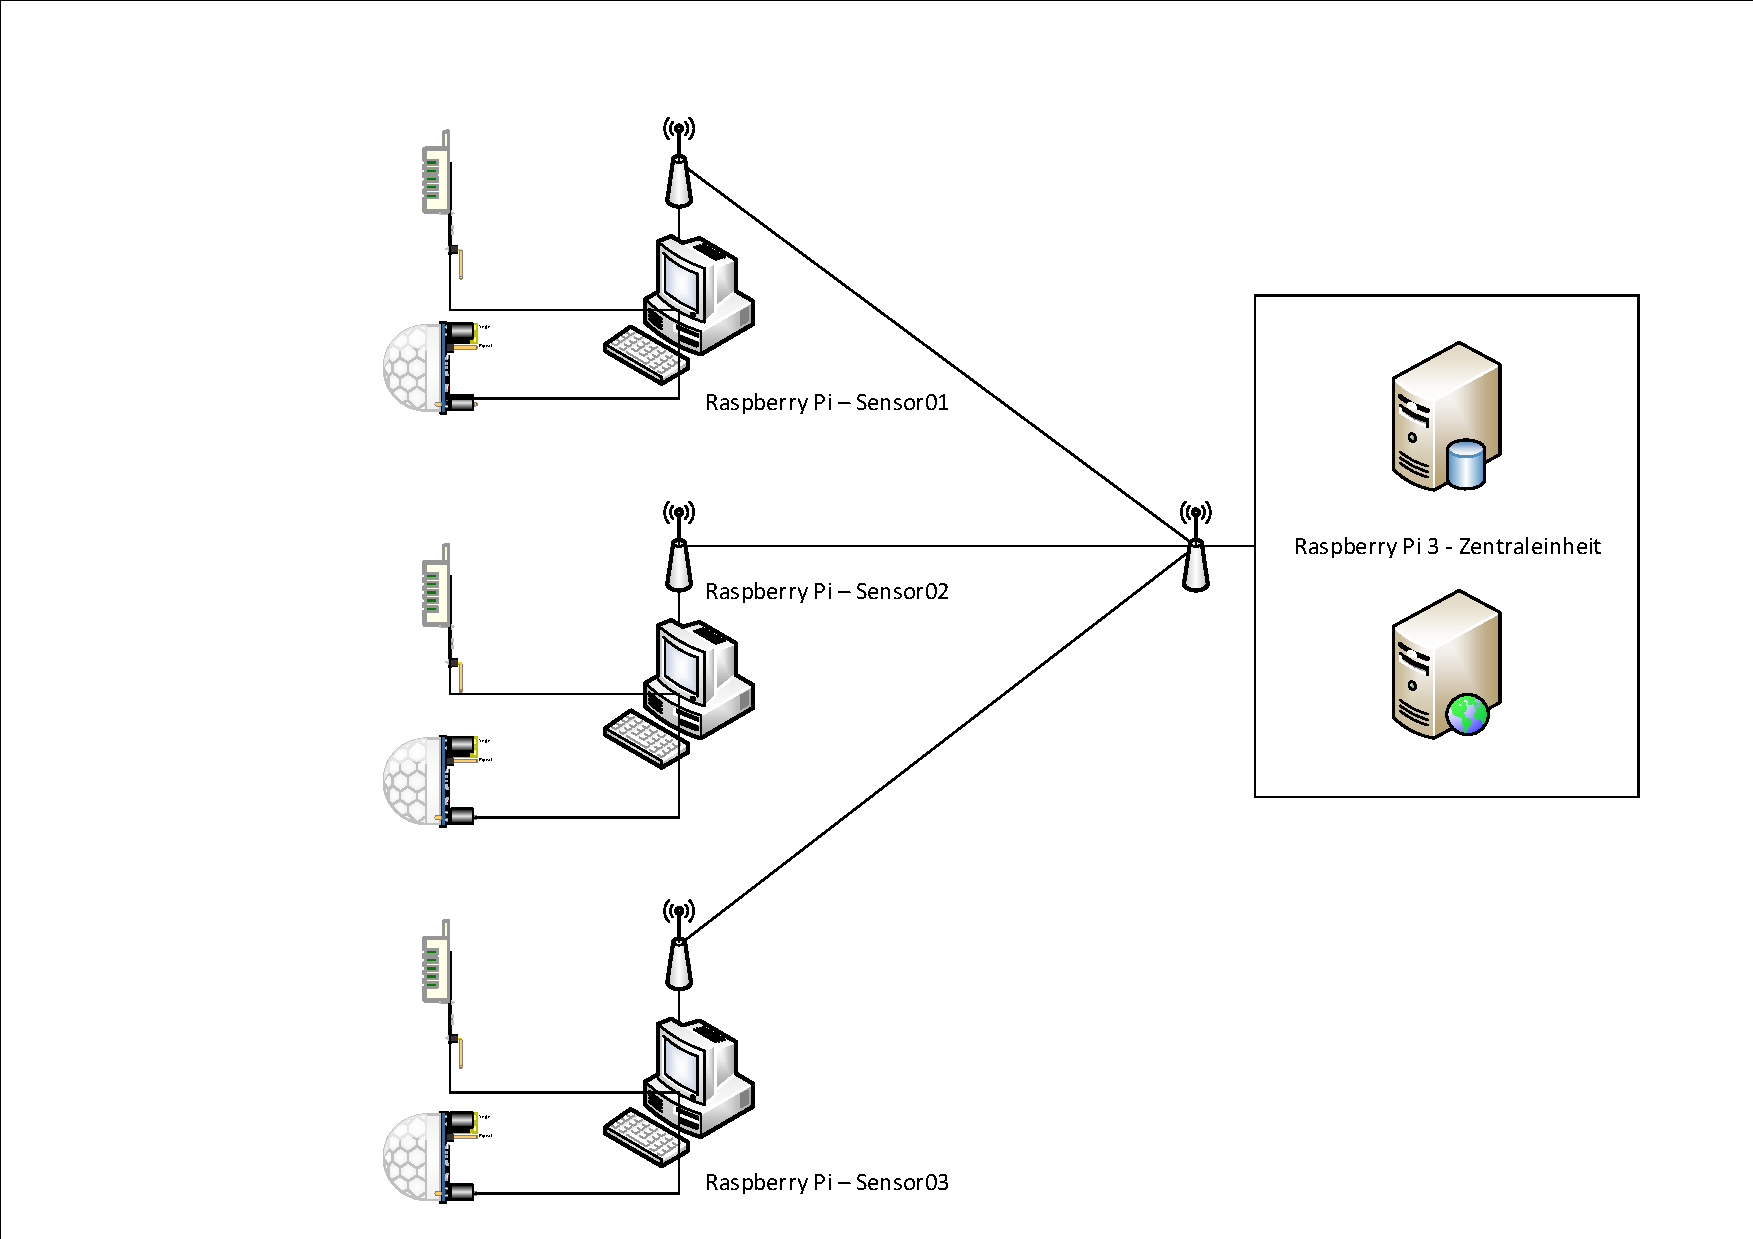
\includegraphics[scale=0.4]{Bilder/Netzplan.pdf}
\caption[Schematische Darstellung der geplanten Umgebung]{Schematische
Darstellung der geplanten Umgebung}
\label{Darstellung_Umgebung}
\end{centering}
\end{figure} 

\section{Website}

Auf der Website kann man sich einloggen und einen neuen Benutzer registrieren.
Nach dem Login kommt man auf eine Übersicht auf der alle Sensorknoten in
Tabellenform abgebildet sind mit den aktuell gemessenen Werten. \\
Auf der Statistik-Seite wird ein Verlauf über mehrere Tage zu einem Sensor
abgebildet.\\
Die Webcam-Seite dient dazu, auf die Webcams zuzugreifen, die an den einzelnen Sensorknoten
angeschlossen sind.\\
Das Impressum dient dazu das Projekt kurz zu beschreiben und dieses Dokument
herunterzuladen.\\
Auf der Logout-Seite bekommt man die Meldung, dass man ausgeloggt ist und die
Möglichkeit zurück zur Login-Seite zu kommen.
(\nameref{Darstellung_Website_einfach})


\begin{figure} [htb]
\begin{centering}
\includegraphics[scale=0.8]{Bilder/struktur_website_einfach.pdf}
\caption[Schematische Darstellung der geplanten Website]{Schematische
Darstellung der geplanten Website}
\label{Darstellung_Website_einfach}
\end{centering}
\end{figure}


\section{Konfiguration}

Die Sensoren werden an einen Raspberry Pi angeschlossen und melden die
gemessenen Werte an einen zentralen Raspberry Pi. Der zentrale Raspberry Pi legt
die gemeldeten Daten in einer Datenbank ab. Eine Website greift auf die
Datenbank zu und stellt die Daten dar.\\
Die Kommunikation wird über ein eigenes WLAN-Netz abgewickelt das von der
Zentraleinheit aufgespannt wird. IP-Adressen werden von einem DHCP-Server, der
auf der Zentraleinheit installiert ist vergeben.\\
Die Website wird durch einen Apache-Webserver auf der Zentraleinheit
bereitgestellt.


\section{Datendiagramme}
xfdtrdzhftjgzjfkzjtderdsfrtdrthztjswtqw
